\documentclass[pdf]{beamer}
\mode<presentation>{}
\usetheme{Frankfurt}


\usepackage{phdGeneral}
\usepackage[utf8]{inputenc}
\usepackage[english]{babel}
\usepackage{hyperref}
%to have greate macro definitions
\usepackage{xparse}
\usepackage{environ} %https://tex.stackexchange.com/a/40043/145331
\usepackage{etoolbox}
%to color text https://texblog.org/2015/05/20/using-colors-in-a-latex-document/
\usepackage{xcolor,soul}
%used to create keystrokes
\usepackage{tikz}
\usetikzlibrary{shadows}
\usetikzlibrary{arrows}
%to use verbatim in boxes
\usepackage{verbatimbox} %https://tex.stackexchange.com/a/120678/145331


%%%%%%%%%%%%%%%%%%%%%%%% CUSTOM AUTHOR AND EMAIL %%%%%%%%%%%%%%%%%%%%%%%%%%%%%

\makeatletter

\global\def\presentation@author{}
\global\def\presentation@email{}

\NewDocumentCommand{\setauthor}{m}{
	\renewcommand{\presentation@author}{#1}%
	\author{\presentation@author \\ \presentation@email}%
}

\NewDocumentCommand{\setemail}{m}{
	\renewcommand{\presentation@email}{\texttt{#1}}%
	\author{\presentation@author \\ \presentation@email}%
}

\makeatother

%%%%%%%%%%%%%%%%%%%%%%%%%%%% ARTICLE MACROS %%%%%%%%%%%%%%%%%%%%%%%%%%%%%%%%%

\NewDocumentCommand{\eg}{}{%
	e.g.,%
}

\NewDocumentCommand{\ie}{}{%
	i.e.,%
}

\definecolor{codeColor}{rgb}{0.952,0.956,0.956}

\NewDocumentCommand{\code}{m}{
	\hl[codeColor]{\texttt{#1}}%
}

\NewDocumentCommand{\mdQuote}{m}{
	``#1''%
}

%%%%%%%%%%%%%%%%%%%%%%%%%%%%%% CENTER WITH CUSTOM SPACE %%%%%%%%%%%%%%%%%%%%%

\NewDocumentEnvironment{parcenter}{O{6pt} O{6pt}}{%
	\parskip=#1\par\nopagebreak\centering%
}{%
	\par\noindent\ignorespacesafterend
}

%%%%%%%%%%%%%%%%%%%%%%%%%%% HIGHLIGHT IN BEAMER %%%%%%%%%%%%%%%%%%%%%%%%%%%%%
%https://tex.stackexchange.com/a/41693/145331

\makeatletter

\let\old@hl\hl
\RenewDocumentCommand{\hl}{O{yellow} m}{%
	\let\set@color\beamerorig@set@color%
	\let\reset@color\beamerorig@reset@color%
	\sethlcolor{#1}%
	\old@hl{#2}%
}

\makeatother

%%%%%%%%%%%%%%%%%%%%%%% CUSTOM BLOCKS %%%%%%%%%%%%%%%%%%%%%%%%%%%%%%%%%%%%%%%%

\newenvironment<>{note}{%
  \begin{actionenv}#1%
      \def\insertblocktitle{Note}%
      \par%
      \mode<presentation>{%
        \setbeamercolor{block title}{fg=white,bg=orange!20!black}
       \setbeamercolor{block body}{fg=black,bg=olive!50}
       \setbeamercolor{itemize item}{fg=orange!20!black}
       \setbeamertemplate{itemize item}[triangle]
     }%
      \usebeamertemplate{block begin}}
    {\par\usebeamertemplate{block end}\end{actionenv}}



%%%%%%%%%%%%%%%%%%%%% TITLE %%%%%%%%%%%%%%%%%%%%%%%%%%%%%%%%%%%%%%

\title{Fundamentals elements of Bash and Linux}
\subtitle{Quick guide to start working with linux}
\setauthor{Massimo Bono}
\setemail{m.bono@unibs.it}
\date{\today}

%%%%%%%%%%%%%%%%%%%% SET SEARH PATHS %%%%%%%%%%%%%%%%%%%%%%%%%%%%%%

\addSrcFolder{{src/texs/}}
\addImagesFolder{{src/imgs/}}
\addTikzFolder{{src/tikzs/}}

%%%%%%%%%%%%%%%%%%%%% CUSTOMIZE BEAMER OUTPUT %%%%%%%%%%%%%%%%%%%%%%

\AtBeginSection[]{
	\begin{frame}<beamer>
	\frametitle{RoadMap}
	\tableofcontents[currentsection]
	\end{frame}
}

\setbeamertemplate{bibliography item}[text]

\beamertemplatenavigationsymbolsempty

\addtobeamertemplate{navigation symbols}{}{%
    \usebeamerfont{footline}%
    \usebeamercolor[fg]{footline}%
    \hspace{1em}%
    \ifbool{is@frame@titleframe}{}{\insertframenumber/\inserttotalframenumber}%
    %\insertframenumber/\inserttotalframenumber
}

%%%%%%%%%%%%%%%%% DOCUMENT %%%%%%%%%%%%%%%%%%%%%%%%%%%%%%%%%%%%%%%%

\begin{document}

\begin{titleframe}
%\renewcommand{\insertnavigation}[1]{}
\titlepage
\end{titleframe}

\section{The shell}

\begin{frame}{What is a shell?}

\begin{block}{Shell}
Simply put, the shell is a program that takes commands from the keyboard and gives them to the operating system to perform\cite{whatIsTheShell}.
\end{block}

\begin{figure}
	\centering
	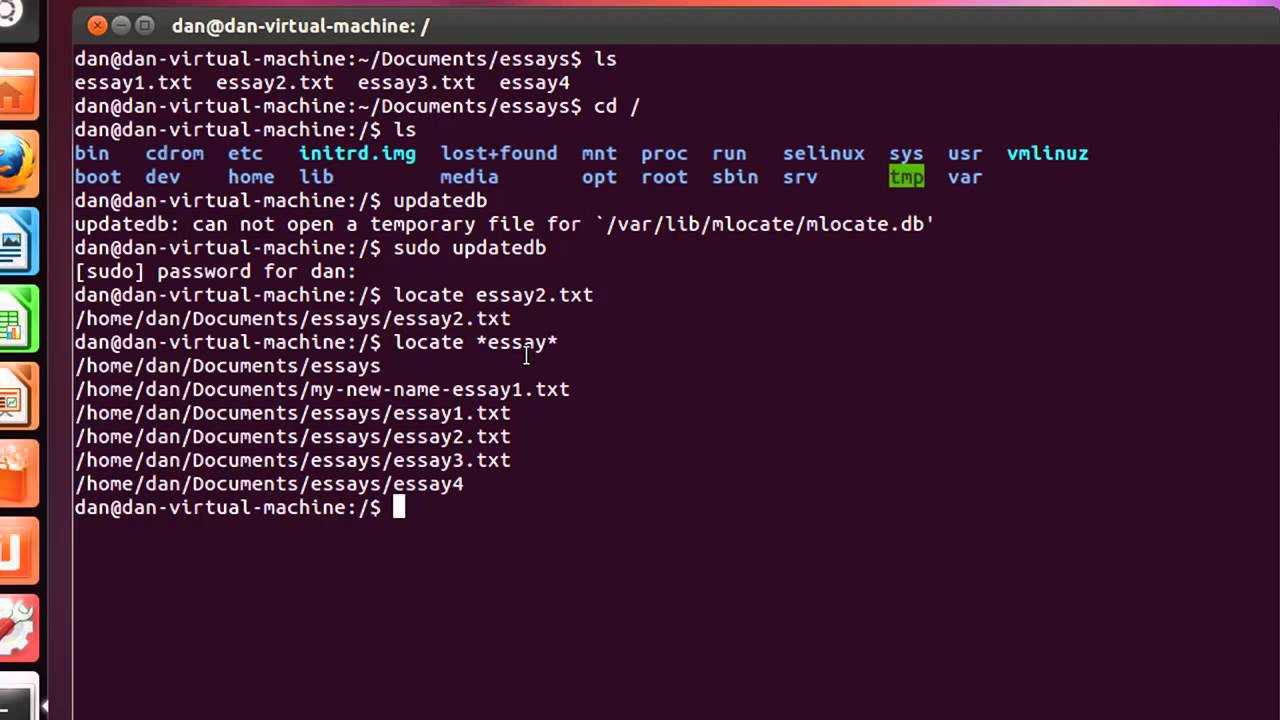
\includegraphics[width=1.0\textwidth]{terminal}
\end{figure}

\end{frame}

\begin{frame}{Shells implementations}
	A shell is an abstract concept. There are several implementations of a \code{shell}. Linux has different shells like \textit{bash}, \textit{sh}, \textit{ksh}. As for Windows, it has \textit{cmd} and \textit{power shell}.
	
	Each shell uses a different syntax for give commands ot the operating system. For instance:
	\begin{itemize}
		\item linux uses \code{ls -l} to print the files within a directory;
		\item windows uses \code{dir} to print the files within a directory;
	\end{itemize}
	
	Shells' syntaxes are theoretically different, but in reality they share lots fo similarities.
	
	\begin{note}
		We will show you \code{bash}, one of the most popular shells in linux.
	\end{note}
\end{frame}

\subsection{Bash: base concepts}

\begin{frame}{Open the shell}
	The shell has different names depending on your operating system. For example:
	\begin{itemize}
		\item Ubuntu: click on Unity bar (top icon on the left side) and type \mdQuote{terminal}. Click the icon to start the terminal \cite{ubuntu:openterminal};
		\item Gnome: \mdQuote{gnome-terminal};
		\item lxUbuntu: \mdQuote{lxterminal};
	\end{itemize}
	
	The shell will start in some directory in your system. For example is may start in \code{/home/your-username/};
\end{frame}

\begin{frame}{Command structure}
	Each command in \code{bash} has the following structure\cite{command:structure}:
	
	\begin{parcenter}[1pt]
		\texttt{command-name command-options command-arguments}
	\end{parcenter}	
	
	For example:
	
	\begin{parcenter}[1pt]
		\code{mkdir -p -v --mode=777 "hello/world"}
	\end{parcenter}
	
	\only<1>{
	\begin{enumerate}
		\item \code{command-name} is the name of the command, in this case \mdQuote{mkdir};
		\item \code{command options} area is an optional part of the command. It represents some flags, options that slightly alter the command behaviour. For example here the options are \mdQuote{-pv --mode=777}.
		\item \code{command arguments} (if any) represents the value the command mainly operate with. They are not prefixed by any \mdQuote{-} character whatsoever. For example \mdQuote{"hello/world"} represents the command arguments.
	\end{enumerate}
	}
	
	\only<2>{
		Options can be typed using 2 conventions: 
		\begin{itemize}
			\item \textbf{brief}(\code{-p}): Typically (but not always) \textit{brief} options have 1 \mdQuote{-} and one character. For example the command has 2 brief options, \code{-p} and \code{-v}. Brief options can be merged: for example typing \mdQuote{-p -v} is always equal (except in few instances) to \mdQuote{-pv}. 
			\item \textbf{long}(\code{--mode}): They are typically (but not always) prefixed by \mdQuote{--}. They are usually composed by more than one character (\ie \mdQuote{mode}).
		\end{itemize}
	}
	
	\only<3>{
		Both \textit{brief} and \textit{long} options can accept arguments. Normally it done using this syntax:
		\begin{itemize}
			\item \textbf{brief}: in general you type the character representing the option, a space and the value of the option (\ie{} \code{-m 777});
			\item \textbf{long}: in general you type the string of the option, a \mdQuote{=} and th value of the option(\ie{} \code{--mode=777});
		\end{itemize}
		
		\begin{note}
			Most options in most commands have both a \textit{brief} and a \textit{long} name. For instance, \mdQuote{-m} and \mdQuote{--mode} for \code{mkdir} commands are synonyms.
		\end{note}
	}
		
\end{frame}

\subsection{Bash: commands}

\begin{frame}{Really basic command}

	\only<1>{
		\begin{block}{man}
			\code{man} stands for \textbf{MANual}. If you want to know all the details about a command, invoke its manual. For example, if you want to know the details of \code{ls}, type \code{man ls}. Basically you type \code{man} followed by a space followed by the name of the command you want to read about. If you don't know the exact syntax of a command, be super sure to check its manual before asking questions! If people, after listening to a question of yours, reply with \mdQuote{RTFM}, it means you should have read the manual (RTFM stands for \mdQuote{\textbf{R}ead \textbf{T}he \textbf{F}unny/\textbf{F}*****g \textbf{M}anual}).
		\end{block}
	}
	
	\only<2>{
		The man contains lots fo useful information: the available options of a command, how to use it, scenarios where it can be successfully used and how to interpret possibly errors.
		
		\begin{note}
			If you want some examples for a particular command, the MAN has them as well! This is why in this presentation we offer no examples whatsoever.
		\end{note}
	}
	
\end{frame}

\begin{frame}{Exercise}

	\begin{enumerate}
		\item<1-> What \code{mkdir} command does?
		\item<2-> Tell me an example of command option (both brief and long);
		\item<3-> How many arguments it can accept?
	\end{enumerate}
	
\end{frame}

\begin{frame}{File system exploration}

	\begin{block}{pwd}
		\code{pwd} will return the \textbf{absolute path} of the directory you're currently in. Super useful if you got lost in the file system.
	\end{block}
	
	\begin{block}{ls}
		returns the list of files (and directories) in the directory you're in. The options of this command tweak the information and the order used to output the content of a directory
	\end{block}
	
	\begin{block}{cd}
		Enters in a subdirectory inside \code{pwd}. Every directory has the directory \code{..}, representing the parent of the directory itself, and the directory \code{.}, representing the directory itself. Hence, the direcotry \mdQuote{/home/koldar/} has a subdirectory called \code{..} pointing to \code{/home/} and a directory called \code{.}, pointing to \code{/home/koldar/}.
	\end{block}

\end{frame}

\begin{frame}{File system manipulation}

	\begin{block}{mkdir}
		Creates a directory in the current working directory.
	\end{block}
	
	\begin{block}{rmdir}
		Remove an empty directory from the file system.
	\end{block}
	
	\begin{block}{rm}
		Remove one or more directories from the file system.
	\end{block}
	
	\begin{block}{touch}
		update to the current time the \mdQuote{last modified date} of a file. Creates the file if it doesn't exist.
	\end{block}
	
	\begin{block}{nano}
		Open a (simplicistic) editor used to alter files. Use \keystroke{Ctrl} + \keystroke{X} to save and exit.
	\end{block}

\end{frame}

\begin{frame}{Exercise}

	\begin{enumerate}
		\item<1-> Create a directory called \mdQuote{hello}?
		\item<2-> Inside it, create a file \mdQuote{world}.
		\item<3-> Inside file \mdQuote{world}, write \mdQuote{hello world};
		\item<4-> save and exit the file.
		\item<3-> Create a copy of \mdQuote{world} file, called \mdQuote{world2}. Use \code{cp} command.
	\end{enumerate}
	
\end{frame}

\begin{frame}{File manipulation}

\end{frame}
\section{Linux}

\begin{frame}{What is linux?}
	\begin{definition}{Linux}
		Linux is the \textbf{kernel} (core) of any operating systems based on Linux.
	\end{definition}
	
	\begin{definition}{Linux distribution}
		A Linux \textbf{distribution} (often called distro for short) is an operating system made as a collection of software based around the Linux kernel.\cite{linux:whatis}
	\end{definition}
	
	Linux distributions are, for example:
	\begin{itemize}
		\item Ubuntu;
		\item Arch;
		\item Lubuntu;
		\item Puppy Linux;
		\item and many, many others;
	\end{itemize}
	
\end{frame}

\begin{frame}{Main components of a Linux distribution}

\begin{figure}
	\centering
	\tikzfile{linuxMainComponents}[0.65]
	\caption{A (incomplete) list of components in a Lnux distribution.\cite{linux:components:sabbagh, linux:components:wiki}}
\end{figure}
	
\end{frame}

\subsection{Users}

\begin{frame}[fragile]{User management}

\begin{block}{Users}
In linux, each users may or may not perform operations on a file/directory. To cope with it, normally we use permission flags (the one returned by \code{ls -l}).
\end{block}

\begin{verbbox}
-rw-rw-r-- 1 root koldar  920 gen 17 14:47 Makefile
\end{verbbox}

\only<1>{
A \mdQuote{group} is a set of users. Each file has 2 associated names: the \textbf{user owning the file} (\textbf{owner}) and the \textbf{the group of the file}.

\fbox{\theverbbox[t]}
	
The file \mdQuote{Makefile} is owned by the user \mdQuote{root} and is associated to the users within the group \mdQuote{koldar}.
}

\begin{verbbox}
-rw-rw-r--  1 koldar koldar  12033 feb  5 16:03 Makefile
\end{verbbox}

\only<2>{
Each permission is a set of about 9 bits:\footnote{There are more than 9 bits, but for clarity we chose to specify only these ones}

\fbox{\theverbbox[t]}

\begin{itemize}
	\item \code{r} stands for \mdQuote{can \textbf{R}ead};
	\item \code{w} stands for \mdQuote{can \textbf{W}rite};
	\item \code{x} stands for \mdQuote{can e\textbf{X}ecute};
\end{itemize}

Each file/directory has 3 sets of these 3 bits:

\begin{enumerate}
	\item one set is applied only to the owner of the file;
	\item one set is applied only to the users in the \textit{group of the file};
	\item one set is applied to everyone else.
\end{enumerate}

}

\only<3>{

\fbox{\theverbbox[t]}

\begin{figure}
	\centering
	\tikzfile{permissionFlags}[0.65]
\end{figure}

Each triple of bits can be seen as a binary number (for example owner bits can be interpreted as 6).

\begin{note}
If \mdQuote{permission denied} happens, it may be the case that your user can't gain access to the file or execute it!
\end{note}

}

\end{frame}

\begin{frame}{Exercise}
	\begin{enumerate}
		\item touch a new file \mdQuote{mario} (see command \code{touch});
		\item use \code{chmod} to prevent \mdQuote{everyone} to \textit{read} the file (last triple of bits);
		\item use \code{chmod} to make \mdQuote{everyone} to \textit{execute} the file (last triple of bits);
		\item (OPTIONAL) use \code{chmod} with the syntax \mdQuote{ugoa+-rwx} to perform the same operation (see \code{chmod} man);
		\item use \code{chown} to change the group of \mdQuote{mario} file to \mdQuote{sudo} (see \code{chown} man);
	\end{enumerate}
\end{frame}

\begin{frame}[fragile]{Root}
	Root is the \textbf{administrator} of your computer, the one which can do \textbf{anything} without worrying about permissions. Sudo has enormous power. Normal users (if permitted) may elevate to root power via (in Ubuntu-like distributions) command \code{sudo}.
	
\begin{verbbox}
echo "Hello world by `whoami`"
sudo echo "Hello wold by `whoami`"
\end{verbbox}
\fbox{\theverbbox[t]}

Question: what the command \code{whoami} does?
	
\end{frame}

\subsection{Package manager}

\begin{frame}[fragile]{Package Manager}

Additional software may be installed on your system. Different Linux distribution uses different package managers.
Ubuntu uses \code{apt-get}.

\begin{verbbox}
sudo apt-get install graphviz
\end{verbbox}
\fbox{\theverbbox[t]}

The above command install the software \mdQuote{graphviz}. Most package manager requires you to have administrator privileges (\code{sudo}).

\begin{verbbox}
sudo apt-get update
\end{verbbox}
\fbox{\theverbbox[t]}

Updates the lists of available packages to install\cite{linux:update:upgrade}

\begin{verbbox}
sudo apt-get upgrade
sudo apt-get dist-upgrade
\end{verbbox}
\fbox{\theverbbox[t]}

Actually perform the new packages installation.

Question: what the command \code{sudo apt-get autoremove} does?

\end{frame}

\begin{frame}{Manual installation}
Some times you need to install software directly from the source. In this case:
\begin{enumerate}
	\item download the source code archive;
	\item look for a file called README or INSTALL;
	\item read such file!
	\item if the above cannot be applied, look for a file called \mdQuote{Makefile}: if present do \code{make \&\& sudo make install};
	\item if the above cannote be applied, look for a file called \mdQuote{configure}: if present do \code{./configure \&\& make \&\& make install};
\end{enumerate}

Question: what the command \code{\&\&} does?
\end{frame}

\begin{frame}[fragile]{File system structure}

\begin{verbbox}
koldar@koldar:~\textdollar ls -l /
total 104
drwxr-xr-x   2 root root  4096 feb  7 12:21 bin
drwxr-xr-x   3 root root  4096 feb  7 12:21 boot
drwxrwxr-x   2 root root  4096 ago  3  2017 cdrom
drwxr-xr-x  19 root root  3940 feb  7 12:19 dev
drwxr-xr-x 141 root root 12288 feb  7 12:21 etc
drwxr-xr-x   3 root root  4096 ago  3  2017 home
lrwxrwxrwx   1 root root    33 gen 25 09:58 initrd.img -> boot/initrd.img-4.4.0-112-generic
lrwxrwxrwx   1 root root    33 gen 11 09:10 initrd.img.old -> boot/initrd.img-4.4.0-109-generic
drwxr-xr-x  22 root root  4096 ago 16 09:34 lib
drwxr-xr-x   2 root root  4096 gen 19 09:12 lib64
drwx------   2 root root 16384 ago  3  2017 lost+found
drwxr-xr-x   4 root root  4096 ago 16 09:25 media
drwxr-xr-x   2 root root  4096 lug 19  2016 mnt
drwxr-xr-x   5 root root  4096 dic 18 20:48 opt
dr-xr-xr-x 191 root root     0 feb  7 12:19 proc
drwx------   5 root root  4096 ott 31 16:40 root
drwxr-xr-x  26 root root   920 feb  7 13:11 run
drwxr-xr-x   2 root root 12288 feb  7 12:21 sbin
drwxr-xr-x   2 root root  4096 giu 29  2016 snap
drwxr-xr-x   2 root root  4096 lug 19  2016 srv
dr-xr-xr-x  13 root root     0 feb  7 12:18 sys
drwxr-xr-x   3 root root  4096 ott 17 09:46 tex
drwxrwxrwt   9 root root  4096 feb  7 19:41 tmp
drwxr-xr-x  11 root root  4096 lug 19  2016 usr
drwxr-xr-x  14 root root  4096 lug 19  2016 var
lrwxrwxrwx   1 root root    30 gen 25 09:58 vmlinuz -> boot/vmlinuz-4.4.0-112-generic
lrwxrwxrwx   1 root root    30 gen 11 09:10 vmlinuz.old -> boot/vmlinuz-4.4.0-109-generic
\end{verbbox}
\scalebox{0.55}{
	\fbox{\theverbbox[t]}%
}

\end{frame}

\begin{frame}[allowframebreaks]
	\frametitle{References}
	\bibliographystyle{plain}
	\bibliography{src/bibs/biblio}
\end{frame}


\end{document}